\documentclass[12pt,twoside]{article}
\usepackage[letterpaper, textwidth=6.5in, textheight=9in]{geometry}
\usepackage{amsmath}
\usepackage{hyperref}
\usepackage{graphicx}

\newcommand{\ve}[1]{\ensuremath{\mathbf{#1}}}

%\newcommand{\vOmega}{\ensuremath{\ve{\Omega}}}
%\newcommand{\hOmega}{\ensuremath{\hat{\ve{\Omega}}}}
%\newcommand{\Ye}[2]{\ensuremath{Y^e_{#1}(\vOmega_#2)}}
%\newcommand{\Yo}[2]{\ensuremath{Y^o_{#1}(\vOmega_#2)}}
%
%\newcommand{\Jij}[2]{\ensuremath{\int L(\vOmega_#1)L(\vOmega_#2)}}
%\newcommand{\Sij}[2]{\ensuremath{\sigma^{gg'}_{\text{s}}(\vOmega_#1 \cdot \vOmega_#2)}}
%
%\newcommand{\sigg}[1]{\ensuremath{\sigma^{gg'}_{\text{s}\,#1}}}
%\newcommand{\psig}{\ensuremath{\psi^g}}
%
%\newcommand{\even}{\ensuremath{\phi^g}}
%\newcommand{\odd}{\ensuremath{\vartheta^g}}
%
%\newcommand{\evenp}{\ensuremath{\phi^{g'}}}
%\newcommand{\oddp}{\ensuremath{\vartheta^{g'}}}
%
%\newcommand{\qe}{\ensuremath{q^g}}
%\newcommand{\qo}{\ensuremath{s^g}}
%
%\newcommand{\apsi}[1]{\ensuremath{\psi^{\dagger\,#1}}}
%\newcommand{\aeven}[1]{\ensuremath{\phi^{\dagger\,#1}}}
%\newcommand{\aodd}[1]{\ensuremath{\vartheta^{\dagger\,#1}}}
%\newcommand{\asigg}[1]{\ensuremath{\sigma^{g'g}_{\text{s}\,#1}}}
%
%\newcommand{\Di}{\ensuremath{\Delta_i}}
%\newcommand{\Dj}{\ensuremath{\Delta_j}}
%\newcommand{\Dk}{\ensuremath{\Delta_k}}
%
%\DeclareMathOperator{\octant}{Octant}

\date{\today}
\title{Notes on Computer Hardware \\and Advanced Architectures}
\author{Rachel Slaybaugh}
%-----------------------------------------------------------
%-----------------------------------------------------------
\begin{document}
\maketitle

\section*{General Memory}

\begin{figure}[!ht]
\begin{center}
  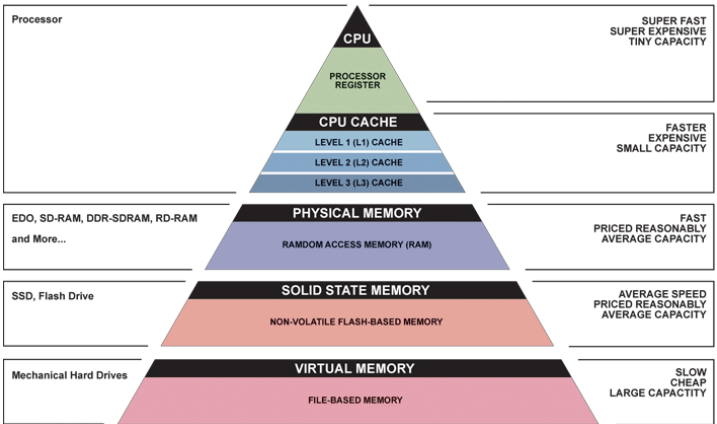
\includegraphics[width=0.8\textwidth, height=0.45\textheight]{cpu-memory-hierarchy}
  \label{fig:cpu-memory}
\end{center}
\end{figure}

Code structure: code is compiled into an assembly program (.s). An assembler turns this into an object, a machine language module (.o). A linker links these and other libraries together into an executable, which is a machine language program (.ext). A loader puts this into memory for execution.

Assembly operands are registers: limited \# of special locations built directly into the hardware (very fast). The MIPS instructions are 32 bits. 

Memory Allocation: \textit{program} (doesn't change size) \rightarrow \textit{static}, variables declared once per program (doesn't change size) \rightarrow \textit{heap}, explicitly created space using e.g.\ malloc \rightarrow \textit{stack}, space for local variables, saved procedure info, etc. (there's a stack pointer that says where this stops.

Once everything is compiled, the machine instructions get translated into memory locations, and switches fire to combine trues and falses (
high/low voltage) to make things actually happen.

In execution, 
\begin{enumerate}
  \item We get the 32-bit instruction word from memory; also increment the program pointer to point to the next instruction. 
  \item Decode the instructions and read the data in the correct registers.  
  \item the Arithmetic-Logic Unit (ALU) does instructions
  \item Then load and store instructions happen and in the cache
  \item results of some computation are usually put into a register.
\end{enumerate}

\textbf{Pipelining Hazards}:
\begin{itemize}
  \item structural hazard: a required resource is busy (e.g.\ needed in multiple stages) 
  \item data hazard: data dependency between instructions; need to wait for previous instruction to complete its data read/write
  \item control hazard: flow of execution depends on previous instruction
\end{itemize}

\end{document}
